\section{Conceptual description}
\label{sec:concept_descr}

An area between the fifth and sixth miles of the Via Appia Antica in Rome is studied and different types of data are collected:
\begin{itemize} 
\item {\em Point clouds (PC)}
    \begin{itemize} 
    \item A low resolution PC of the studied area that has been generated making
    use of Fugro's DRIVE-MAP services.
    \item High resolution PCs of the different monuments generated using photogrammetric technologies.
    \end{itemize}
\item {\em Meshes} reconstructions (3D models) of the monuments for different historical epochs.
\item Contemporary and historical {\em pictures} or paintings.
\item Footprints in 2D of the monuments acquired using Topcon positioning systems. 
\item {\em Attributes} data for the monuments and their parts, which are gathered
by field observations.
\end{itemize}

We conceptually divide the area into items and there are two types of items:
\begin{itemize}
\item \textit{background}: It is the whole area considered as one single entity (item).
\item \textit{sites}: The different monuments of interest contained in the area. They are considered as different entities (items)
\end{itemize}

The point clouds, meshes and pictures are stored according to the data
structure defined in section \ref{sec:data_structure}. In the next subsections we provide more information of the different types of data and we specify to which type of item they are related according to the previous conceptual definition. 

\subsection{Point clouds}

Different types of point clouds are collected and handled

\subsubsection{DRIVE-MAP}

Using the DRIVE-MAP service of Fugro the the road was scanned and a
{\em PC} was produced. A point in the PC has 3D coordinates ($x, y, z$), in
respect to a given Earth reference system known at scanning time, and it also has color and
other attributes as classification. The resolution (number of points per area
or volume) of this point cloud is not enough to see detailed features of the
sites. Furthermore, they were only scanned from the main road. Thus, the back
of the sites is missing. This is illustrated on Fig.\ref{fig:viaAppiaPointCloud}.

\begin{figure}[!ht] \centering
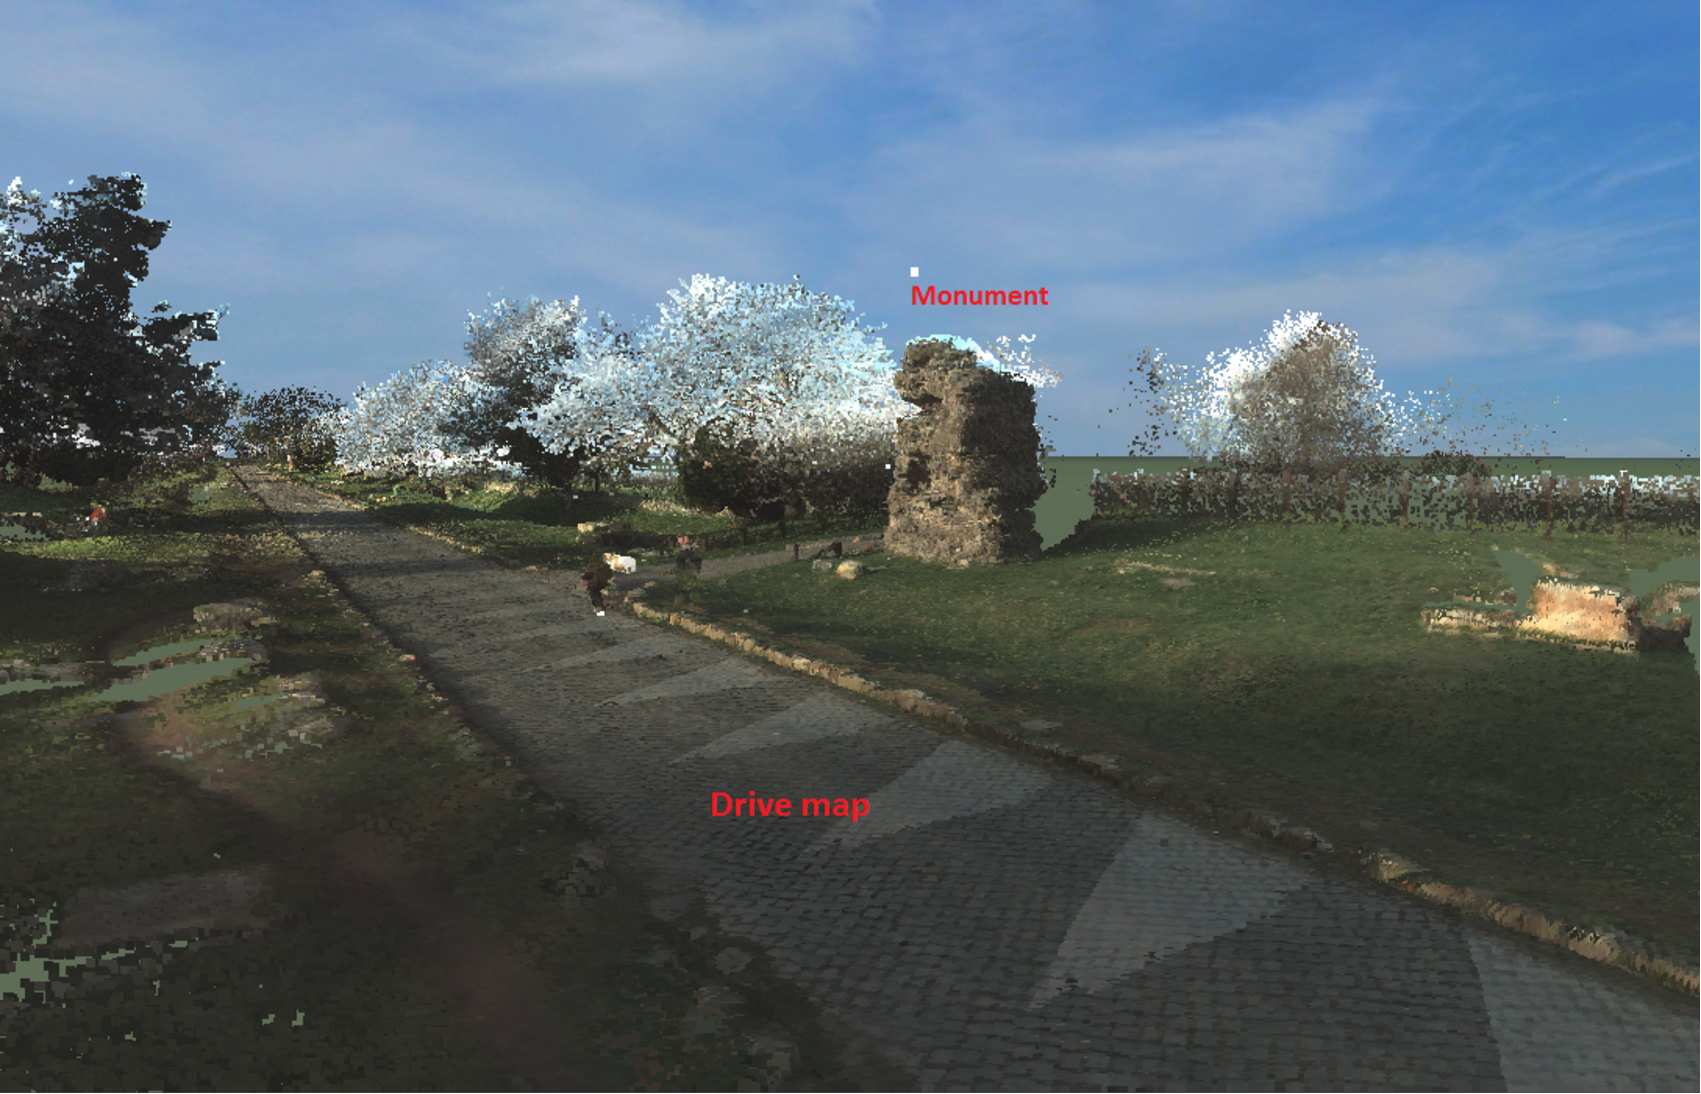
\includegraphics[scale=0.5]{fig/conceptual_description/ViaAppiaPCAnnot.pdf}
\caption{Point cloud data gathered along Via Appia. The Drive map is of low
resolution and covers only part of the monuments (sites) facing the road.}
\label{fig:viaAppiaPointCloud} \end{figure}

There are different versions of the same DRIVE-MAP, each version contains different processed point clouds. For example, there is a version where the points from some trees have been removed (using the classification attribute of the points).

The DRIVE-MAP dataset is \textit{background} data.

\subsubsection{Photogrammetry}

Additional point clouds of higher resolution covering also the back of the
monuments have been obtained using photogrammetric software from photographic
pictures of the sites from different camera locations (viewpoints). Such point clouds are \textit{sites} data.

\subsection{Pictures}
There are several pictures of the sites, both contemporary (current) and historical pictures or paintings. Fig.\ref{fig:viaAppiaMeshPicture} has an illustration of visualizing
a contemporary photo of a monument next to its point cloud data. The photo was
one of the photos used to generate the high resolution site PC and visualizing
it next to the location of the monument provides extra information about the
context. Each site has multiple pictures. The sites pictures are \textit{sites} data.

\subsection{Meshes}
For the purpose of archaeological research, multiple reconstructions of the
sites of interest are often performed. These reconstructions, or meshes, are
also classified as current or historical. An illustration of visualizing a
contemporary mesh of a monument aligned to its point cloud data is pictured
on Fig.\ref{fig:viaAppiaMeshPicture}. The different meshes are \textit{sites} data.

\begin{figure}[!ht] \centering
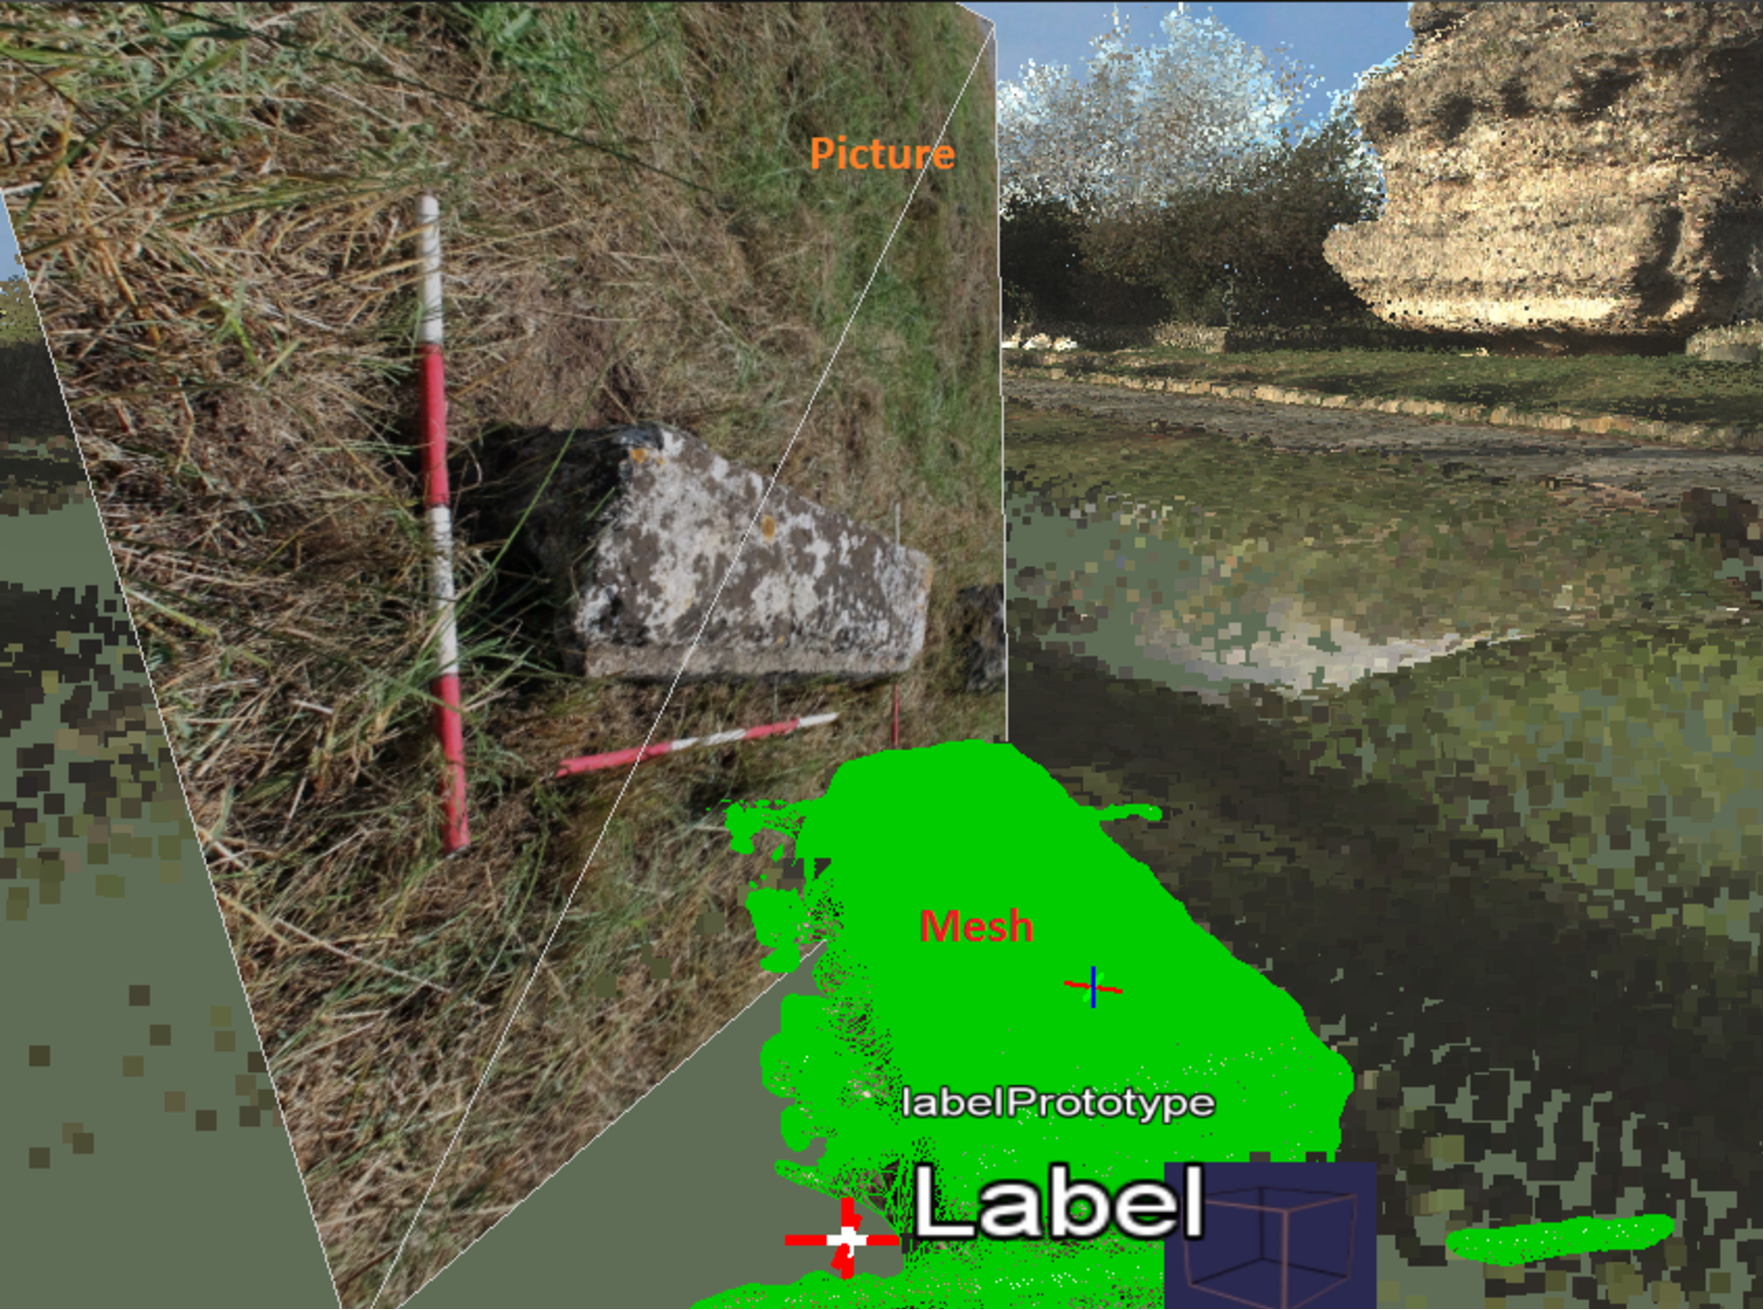
\includegraphics[scale=0.5]{fig/conceptual_description/ViaAppiaMeshPicture.pdf}
\caption{Reconstruction meshes and picture of a site overlayed on the point
cloud data.} \label{fig:viaAppiaMeshPicture} \end{figure}

\subsection{Footprints}
Topcon 2D footprints were also collected for the different sites in the area. This data is geo-referenced. This is \textit{sites} data.

\subsection{Attributes}
Attributes represents the data collected at the site by the archaeologists, 
for example, material composition, condition, possible interpretation,
description of the different elements or sub-parts, etc. The attribute data
is considered as additional descriptive (meta) data and it is stored in a
database along with the pointers to the other data types (Section
\ref{sec:database}). Furthermore, they are extremely relevant for the definition
of archaeological research questions. This is \textit{sites} data.
